%%%%%%%%%%%%%%%%%%%%%%%%%%%
%%% Chapter definitions %%%
%%%%%%%%%%%%%%%%%%%%%%%%%%%
% Chapter title
\renewcommand{\mychaptertitle}{%
Dramatic change in drag\\ by catastrophic phase inversion
}
% Chapter short title
\renewcommand{\mychaptershorttitle}{%
Dramatic change in drag by catastrophic phase inversion
}
% Chapter authors
\renewcommand{\mychapterauthors}{%
\textbf{Dennis~Bakhuis},
Rodrigo~Ezeta,
Pim~A.~Bullee,
Sander~G.~Huisman,
Alvaro~Marin,
Detlef~Lohse,
and
Chao~Sun
\textit{Dramatic change in drag by catestrophic phase inversion},
manuscript in preparation.
}
% Chapter abstract
\renewcommand{\mychapterabstract}{%
In this letter we investigate oil-water mixtures in highly turbulent
Taylor--Couette flow.
In the absence of an emulsifier, energy-input from the
turbulence provides the energy to continuously break-up droplets, such that
the phases do not separate.
We show how a mixture of oil and water can have
effective viscosities larger or smaller than each species.
In addition, we
report on the catastrophic phase-inversion of these mixtures, with its
concomitant drop in effective viscosity.
We find that for a fixed
oil fraction we can have either a water-in-oil or
oil-in-water mixture with vastly different droplet sizes and rheological properties.
The manifestation of
these states is exemplified by providing combined local and global
measurements of highly turbulent oil-water mixtures in the Twente Turbulent
Taylor--Couette facility, including in-situ microscopy imaging.
We explain our findings due to the different nature of droplet size
distributions and associated deformability.
Our findings demonstrate that using an optimal mix of two immiscible fluids can lead to drastic
energy reductions while exceeding this optimum will lead to the opposite.
}
\renewcommand{\mychaptermark}{Emulsions}
\renewcommand{\mychapterlabel}{chap:emulsions}
\renewcommand{\mychaptericon}{fig/swchapter3.png}
%%%%%%%%%%%%%%%%%%%%%%%%%%%%%
%%% Create Chapter Header %%%
%%%%%%%%%%%%%%%%%%%%%%%%%%%%%
%%%%%%%%%%%%%%%%%%%%%%
%%% Chapter header %%%
%%%%%%%%%%%%%%%%%%%%%%
\globalcolor{ChapterText}
\chapter[\mychaptershorttitle]{%
    \mychaptertitle%
    \ifdefined\starwarsfootnotes
        \textsuperscript{%
            \hspace{-1mm}%
            \includegraphics[height=\swsymsize]{\mychaptericon}%
        }%
        \blfootnote{%
            \textcolor{footnotetextcolor}{%
                \textsf{%
                    \vspace{0.5mm}\hspace{-1mm}%
                    \includegraphics[height=\swfnsymsize]{\mychaptericon}%
                    \hspace{0.5mm}%
                    Based on: \mychapterauthors%
                }
            }
        }
    \else
        \footnote{\textsf{%
             Based on: \mychapterauthors%
        }}%
    \fi
}
\pagecolor{ChapterBackground}
\afterpage{\pagecolor{White}\globalcolor{Black}} 
\label{\mychapterlabel}
\chaptermark{\mychaptermark}
\noindent\rule{\textwidth}{0.4pt}%
\vspace{0.2cm}
\noindent\textsf{\mychapterabstract}
\clearpage

%%%%%%%%%%%%%%%%%%%%%%%%
%%%% end title page %%%%
%%%%%%%%%%%%%%%%%%%%%%%%
\graphicspath{{ChapterThree/fig/}}

\ifdefined\thesissections%
\section{Introduction}%
\fi%
% Why important
Mixtures of oil and water are omnipresent in petro-chemical processes,
biological systems, as well as in the food industry.
For oil recovery, for example, water is generally used as a carrier liquid to extract oil
from the ground creating an emulsion. In food industry emulsions are generally found in all sorts of products together with stabilizers \,\cite{mcClements2004}.
% Why immiscible
Due to their polar and non-polar nature, water and oil are immiscible.
% Definition of emulsions
Although by definition immiscible fluids cannot be mixed, they can be dispersed into each other by vigorously shaking or stirring. One phase is typically fragmented in the form of drops (becoming the dispersed or internal phase) and suspended inside the
other fluid (\text{i.e.} the continuous or external phase), thereby, creating
an emulsion.
% Definition morphologies: w-o / o-w
Emulsions can be categorized in two morphologies types: simple emulsions and multiple emulsions\,\cite{Becher2001}.
Simple emulsions are oil droplets suspended in water (o--w) or water droplets suspended in oil (w--o).
% Alvaro says: I don't see why should we introduce multiple emulsions, right?
% A multiple emulsion can be seen as an emulsion inside an emulsion, for which their are again two possibilities: oil droplets in water droplets in oil (o--w--o) and water droplets in oil droplets in water (w--o--w).
% Stability and emulsifiers
An emulsion can become easily unstable, typically by coalescence of the disperse phase
as a result, the two phases completely separate. Depending on the application, emulsifiers
(surfactants and/or polymers) can be added to gain stability against coalescence.
% [Often the dispersed droplets easily coalesce, especially under the influence of buoyancy due to their different densities, and, --> Alvaro says: that was too specific]
% Phase inversion -> Alvaro says: watch out, with some emulsifiers, specially polymers, there might be no phase inversion
As the dispersed phase volume fraction is increased, a phase
inversion might occur in which dispersed and continuous phases  
switch roles\,\cite{Salager2000, Perazzo2015}.  There are various attempts to model
the phase inversion: continuous drops trapped in multiple
emulsions\,\cite{Pal1993, Jahanzad2009}, minimal dissipation
model\,\cite{Poesio2008, Ngan2009}, energy barrier model\,\cite{Piela2009}, or
a coalescence/breakup model\,\cite{Brauner2002,Yeo2002}. 
% Catastrophic
A phase inversion process can occur at very different time scales: it can take up to days when it occurs due to gravitational effects (sedimentation or flotation of the dispersed phase), or it can occur instantaneously. The latter scenario is typically called a \emph{catastrophic phase inversion}\,\cite{Dickinson1981, Vaessen1996, Tyrode2005}.
% Ambivalence region
The critical inversion point of o--w and w--o are generally not at the same oil volume fraction and hysteresis is observed\,\cite{Brauner2002,Yeo2002,Piela2006, Moradpour2011}.
It was found that width of the hysteresis region, also known as the ambivalence
region, is a unique property of the emulsion mixture and independent of
Reynolds, Froud, and Weber number\,\cite{Piela2009}
% Emulsions in turbulence
The break-up of droplets in a turbulent flow was pioneered by
Kolmogorov\,\cite{Kolmogorov1949} and Hinze\,\cite{Hinze1955}.
Their focus was to determine a correlation between the flow scales and the average droplet diameter by dimensional analysis.
Turbulent eddies with a scale similar to the droplet can destabilize the interfaces, leading to the break-up of droplets\,\cite{Andersson2006}.
% [sometimes splitting them in half -> Alvaro says: "in half"? that's very specific]
While the smallest scale in a turbulent flow, \text{i.e.} the Kolmogorov scale $\eta_K$, was hypothesized as the lower bound for the droplet diameter, a large portion of droplets can have a smaller size\,\cite{Zhou1998}.
At these scales (viscous subrange), subeddy viscous stresses dominate over
inertial stresses, making smaller droplets possible\,\cite{Shinnar1961,
Boxall2011}.
% Dynamic equilibrium
In a turbulent flow, without any surfactant or emulsifier, a dynamic equilibrium emerges: the energy-input of the turbulence continuously
provides energy to break up droplets, while the droplets continuously merge and coalesce. Stopping the energy input quickly destroys the equilibrium and the phases separate. 
% However, due to their size and density difference these drops can be considered as `inertial particles', making it more likely for them to cross trajectories of other drops, resulting in an increased chance of coalescence.
% Rheology and link with drag
Adding inclusions such as solids, gas or immiscible fluids to a liquid can
dramatically change its rheology\,\cite{Derkach2009, Stickel2005}. Solids generally increase the effective viscosity\,\cite{Bakhuis2018}, while
small amounts of polymers \cite{White2008}, oil without
surfactant\,\cite{Pal1993}, or gas\,\cite{vanGils2013,Verschoof2016} are known to reduce drag, yielding a lower effective viscosity as the original liquid phase.
% Link to Weber number
For the case of air-lubrication, the current understanding
suggests\,\cite{Verschoof2016, vanGils2013, Spandan2018} that the requirement
for large drag reduction is the deformability (expressed as the Weber number) of
the gas phase.\\
\ifdefined\thesissections%
\section{Experiments and results}%
\fi%
% Problem description
% [investigate the effective viscosity $\nu_\text{eff}$--> Alvaro says: that's more the method you use, not the aim of the study.]
% Alvaro says: maybe "dynamic phase stability" is too broad, we could consider saying "flowing properties"? I don't like it either...
\indent In this \docname we investigate the dynamic phase stability of a meta-stable emulsion without surfactants, in a highly turbulent shear flow. For doing so, we measure the effective viscosity effective viscosity $\nu_\text{eff}$ of the turbulent emulsion. 
Viscosities of meta-stable emulsions (MSE) can not be easily measured in the laminar regime, as the phases would quickly separate. To keep the MSE mixed, a turbulent flow is required. Unfortunately, conventional rheometers work in predictable flow regimes and therefore they can only operate in the laminar regime. Recent advances\,\cite{Grossmann2016} in turbulent Taylor--Couette (TC) flows makes it possible to use this geometry as a rheometer---classically solely used in the laminar regime---even in the turbulent regime.
% Setup
For all measurements we make use of the Twente Turbulent Taylor--Couette
(T${}^3$C) facility\,\cite{vanGils2011}, as this provides local and global
measurement access in a controlled and closed geometry (schematic shown in
\reff{fig:setupoil}A).
%
\begin{figure}
\centering
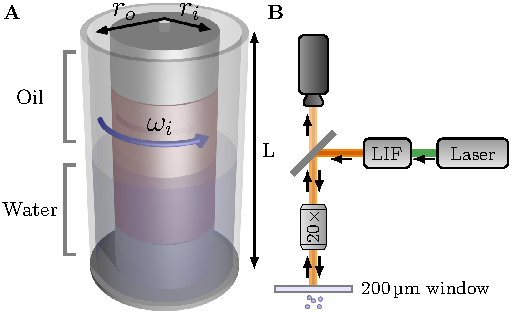
\includegraphics{SetupSchematic.pdf}
\caption{%
A. Schematic of the T$^3$C setup.
Initially, the water (bottom) and oil(top) are separated.
B. In-situ high-speed microscopy using LIF lighting, a
half-mirror, and a $20\times$ magnification lens, through a \SI{200}{\micro\meter}
thick window at the top of the setup shown in A.%
}
\label{fig:setupoil}
\end{figure}%
%
The apparatus has an inner cylinder (IC) radius $\ri=\SI{200}{\milli\meter}$,
an outer cylinder (OC) radius of $\ro=\SI{279.4}{\milli\meter}$, and a height
of $L=\SI{927}{\milli\meter}$, resulting in a gap width
$d=\SI{79.4}{\milli\meter}$, a radius ratio of $\eta=\ri/\ro=0.716$, and an
aspect ratio $\Gamma=L/d = 11.7$.
The torque, $\mathcal{T}$, required to rotate the IC at constant angular
velocity $\omegai$ is measured using a hollow reaction torque sensor,
while the temperature is kept at \SI[separate-uncertainty =
true,multi-part-units=single]{21.0(5)}{\celsius}.
Optical access to the flow is through a window on top of the system, modified
to hold a \SI{200}{\micro\metre} glass plate, thereby, allowing to operate a
microscopy system~(shown in \reff{fig:setupoil}B).
The microscopy system consists of laser-induced fluorescence lighting (LIF),
a half-mirror, $20\times$ magnification lens, and two cameras: Lumenera LM165 and Photron SA-Z.
% Type of oil
We make use of demineralised water and a low-viscosity silicone oil\,\cite{ShinEtsuKF96} with
$\nu_o=\SI{1.03}{\milli\meter\squared\per\second}$ at $\SI{25}{\celsius}$ and an interfacial tension with water of $\gamma =\SI{42.7}{\milli\newton\per\metre}$\,\cite{Kanellopoulos1971}.\\
% Ta / Nuw
\indent The driving of TC flow can be characterized by the Taylor
number\,\cite{Eckhardt2007}:
\begin{align}
    \text{Ta} = \frac 14 \sigma d^2 (\ri + \ro)^2 (\omegai - \omegao)^2 /
    \nu^2
    \label{eq:oilTa}
\end{align}
where $\sigma = ((1+\eta)/(2\sqrt \eta))^4$ is a geometric constant.  The
output of the system, the torque, can then be captured as a $\omega$-Nusselt
number:
\begin{align}
    \text{Nu}_\omega \equiv  \frac{J_\omega}{J^{\text{lam}}_{\omega}} =
    \frac{\mathcal{T}}{2\pi L \rho J^{\text{lam}}_{\omega}}.
    \label{eq:oilNu}
\end{align}
Here $J^{\text{lam}}_{\omega} = 2 \nu \ri^2 \ro^2(\omegai - \omegao)/(\ro^2 - \ri^2)$ is the angular velocity transport for laminar, non-vortical flow and the angular velocity of the OC is $\omegao=0$.
From previous studies\,\cite{vanGils2011b,Paoletti2011,Huisman2012b, Ostilla-Monico2014b, Huisman2014,Grossmann2016}
we know that $\text{Nu}_\omega=f(\text{Ta},\eta,\omegai/\omegao)$.
In order to compute an effective viscosity for the MSE, we will assume that it responds as a Newtonian liquid at these shear rates. 
% Torque(fic) measurements
While quasi-statically driving the inner cylinder for
$\omegai/(2\pi)=4$--$\SI{20}{\hertz}$,
$\mathcal{T}$ was measured for various oil volume fractions
$\alpha=V_o/(V_o+V_w)$, where $V_o$($V_w$) is the volume
of the oil(water) phase. Experiments based on liquids with known viscosity defines the curve $\Nuw=f(\Ta)$ for our geometry, which we do so using the $\alpha=\SI{0}{\percent}$ and $\alpha=\SI{100}{\percent}$ cases and exploiting the known scaling\,\cite{Lathrop1992,vanGils2011b,Paoletti2011}. This scaling in the ultimate regime, $\Nuw=f(\Ta)$, can now be exploited to determine $\nue(\alpha)$ such as to collapse all the data on to a single curve, see the collapsed data of 32 experiments in \reff{fig:torqueoil}.
%
\begin{figure}[t]
\centering
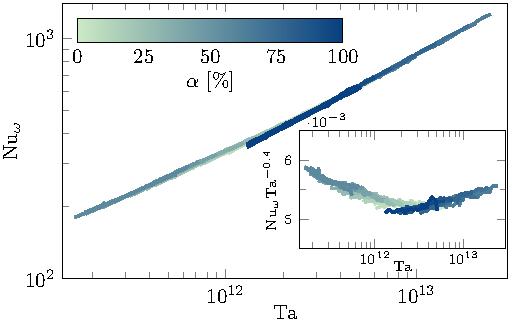
\includegraphics{tavsnuw.pdf}
\caption{%
    Exploiting the relation between $\Nuw=f(\Ta)$, a $\nue$ was found such
    that 32 datasets share a single curve, by minimizing $\sigma(\Nuw)$ for the
    collective data, binned in $\Ta$. The result of this minimization is shown
    as the closest to a single curve for all sets, for $\Nuw$. The inset shows
    the same datasets, compensated using $\Ta^{0.4}$, revealing the overlap
    within a couple of percent.
}
\label{fig:torqueoil}
\end{figure}%
%
% [Alvaro says: I removed the "As expected", since we don't know if it should behave as Newtonian!]
All datasets collapse onto a single universal curve, consistent
with previous studies on Newtonian liquids\,\cite{Lathrop1992,vanGils2011b, Ostilla-Monico2014b}.
To appreciate the quality of the collapse, all data is compensated by
$\Ta^{0.4}$ (inset of \reff{fig:torqueoil}), which shows that all
datasets have an error of \SI{1.2}{\percent} and justifies the
Newtonian assumption made earlier for the MSE at such large shear rates.\\
% Effective viscosity
% [Alvaro says: I removed "from the \emph{static} measurements" because you have not explained yet what does it refer to. It's just confusing]
\indent The effective viscosity $\nue(\alpha)$, normalized using the viscosity of water $\nu_w$ (all at
\SI{21}{\celsius}) are shown in \reff{fig:viscosity} as blue
circles.  Each experimental measurement in this set is performed at constant oil fraction  $\alpha$, and therefore is depicted as \emph{static} $\alpha$ in the plot. 
Remarkably, we observe two disconnected branches, the left
branch for $\alpha \leq \SI{65}{\percent}$, and the right branch for
$\alpha\geq \SI{70}{\percent}$.
%
Starting from pure water, adding oil (\circled{a}) increases the effective
viscosity beyond the viscosities of each of the constituents, making the fluid
three times as viscous for $\alpha=\SI{65}{\percent}$.  Further increasing
$\alpha$ in excess of \SI{65}{\percent} results in a dramatic drop in $\nue$.
This is caused by a phase inversion; whereas for $\alpha \leq 65\%$ we had
o--w, for $\alpha \geq 70\%$ we have w--o, showing a tremendous change in
rheology.
% Drag reducing effect
When starting from pure oil, adding water (\circled{b}) lowers the effective
viscosity, and thereby, resulting in drag reduction.  For
$\alpha=\SI{70}{\percent}$, the torque is \SI{13}{\percent} lower as for pure
oil, similar to other w--o emulsions\,\cite{Pal1993}.  For the present regime
of $\Ta = \mathcal{O}(10^{11}$--$10^{13})$, one can derive that
$\mathcal{T}_\text{o}/\mathcal{T}_\text{w} \propto (\nu_o/\nu_w)^{0.2}$, and
from this we, indeed, find a $\nue$ approximately half the value of pure oil
for $\alpha=70\%$.
% Dynamic measurements: adding oil
At phase inversion, $\nue$ decreases (or increases) by a factor 6,
resulting in a tremendous change of more than \SI{40}{\percent} in torque.
To further investigate what is happening at phase inversion we now
quasi-statically increase $\alpha$ by slowly draining the setup at the bottom
while filling it with oil from the top, see the red
curves($\dif{\alpha}/\dif{t} > 0$) in \reff{fig:viscosity}.
For all of these \emph{dynamic} experiments, $\omegai/(2\pi)$ was fixed to
\SI{17.5}{\hertz} and the mass of the injected liquid was recorded.
The instantaneous value of $\alpha$ is obtained taking into account the injected liquid and assuming that the liquid drained is an homogeneous mixed emulsion.
At the end of the experiment, $\alpha$ was directly measured and found to be within
\SI{1}{\percent} of the calculated value.
Here, we observe a displaced \emph{catastrophic} phase inversion at
$\alpha=\SI{72}{\percent}$ (\circled{\footnotesize{J1}}), exceeding 
$\alpha$ from the \emph{static} measurements.
%
\begin{figure}[t]
    \centering
    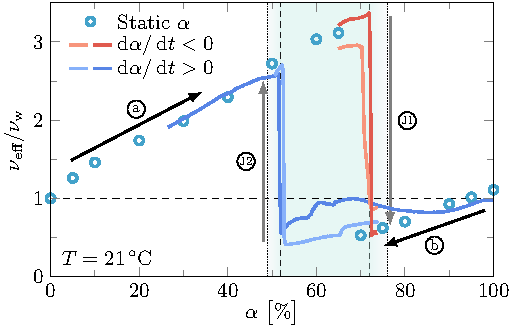
\includegraphics{viscosityfit.pdf}
    \caption{%
    Effective viscosity normalized by the viscosity of water as function of
    oil volume fraction. The static measurements where the fluid is premixed
    are shown by circles. The continuous measurements, for which $\alpha$ is
    changed during the experiments ($\omega_{ic}/(2\pi)$ is fixed at
    \SI{17.5}{\hertz}), are shown solid lines.
    The shade area shows
    the ambivalence area, bounded by two catastrophic phase inversion,
    \circled{\footnotesize{J1}}: w--o $\rightarrow$ o--w and
    \circled{\footnotesize{J2}}: o--w $\rightarrow$ w--o. When water is the
    continuous phase, increasing $\alpha$ leads to an increase in $\nue$
    (\circled{a}), while for oil, increasing the water
    fraction, decreases $\nue$ (\circled{b}).
    When $\omegai$ is decreased, the
    ambivalence region increases in width (indicated by dashed to dotted
    boundary).
    }
    \label{fig:viscosity}
\end{figure}
% Dynamic measurements: adding water
The reversed experiment, slowly decreasing $\alpha$ by filling the system with
water and draining the mixed emulsion, results in the opposite
\emph{catastrophic} phase-inversion, see the blue curves
($\dif{\alpha}/\dif{t} < 0$) in \reff{fig:viscosity}.
The torque measured by the inner cylinder sharply increases with more than
\SI{35}{\percent}, switching from drag reduction to a severe drag increase
slightly around $\alpha=\SI{50}{\percent}$.
% catastrophic
What is striking is that the change in morphology at
\circled{\footnotesize{J1}} and \circled{\footnotesize{J2}} happens instantaneously.
The dispersed phase exceeds the critical amount and triggers a phase
inversion resulting in a very different rheology of the MSE.
The effects are instantly visible in the measured torque of the system, but
also in the temperature, as the active cooling of the setup needs immediate
adjustments.
% Repeating dynamic measurements
Repeating the \emph{dynamic} measurements, indicated by shaded colors in
\reff{fig:viscosity}, we observe that the critical $\alpha$ (amount of
dispersed phase required to get phase inversion) is very reproducible.
% Ambivalence region
Note that the volume fraction for the transition from w--o to o--w
(\circled{\footnotesize{J2}}) is distinctly different from the o--w to w--o
(\circled{\footnotesize{J1}}) case.
Here, the MSE shows a hysteretic morphology, in the an ambivalence region,
$\SI{52}{\percent} \leq \alpha \leq \SI{72}{\percent}$ (shaded blue area
shown in \reff{fig:viscosity}), even for such high Reynolds numbers of
$\mathcal{O}(10^6)$.
One would naively think that for such a high Reynolds number the system
provides ample power to trigger any instability, however it has been shown
before that turbulent TC flow is susceptible to hysteresis\,\cite{Huisman2014,
vanderVeen2016}.
% Multiple states
Also noteworthy is that in the ambivalence region, each morphology can
have multiple values for $\nue$ as there is some discrepancy between the
repeated measurements.
We expect the distribution of droplet sizes differ slightly between the
measurements which can have a large impact on the rheology\,\cite{Pal1996}.
% small Re effect on ambivalence region
%
Catastrophic phase inversion has been also observed in turbulent pipe flows\,\cite{Piela2006,Piela2008}, in which the width of the ambivalence region is solely dependent on the ratio of the dispersed phase injection rate and the 
total flow rate.  In our case, we have a dispersed phase
injection rate of approximately \SI{12.5}{\milli\liter\per\second}, which can
either be water or oil.
We do, however, observe that the ambivalence region gets slightly
wider when $\Ta$ is decreased (illustrated from dashed to dotted boundaries in
\reff{fig:viscosity}).
The ambivalence region increases by a couple percent on both sides, thereby
displacing the phase inversion for each morphology.
% Why droplet size
The different response seen on the left and right branches in Figure \ref{fig:viscosity} demands a detailed
look of the flow. The decrease in $\nue$ for w--o emulsions (\circled{b})
could be a similar process as in bubble drag
reduction\,\cite{vandenBerg2007,Verschoof2016}, related with the deformability of the dispersed phase, for which large droplets are required.  Using the same reasoning, an
increasing $\nue$ (\circled{a}) should be connected with the presence of small and non-deformable droplets which would act as solid-like particles and therefore increase
$\nue$\,\cite{Stickel2005,Bakhuis2018}.
% droplet size setup
Consequently, we could explain the observed changes in viscosity by analyzing the droplet distribution. However, due to the metastable nature of the mixture, the emulsion quickly separates when energy is not supplied, and therefore we cannot guarantee that samples taken from the system and analyzed under a standard microscope have the same morphology as those flowing in the system at high energy. Consequently, we choose for bringing the microscope to our apparatus and size the dispersed phase while flowing. The
optical system arranged is shown in \reff{fig:setupoil}B. Note that the dispersed droplets are visualized by the reflected light from their interface and that no fluorescent dye was employed. The MSE was premixed
(\emph{static}) at $\alpha=\SI{60}{\percent}$ and the IC was fixed to an
angular velocity $\omegai/(2\pi) = \SI{8}{\hertz}$. For this $\alpha$, we are
approximately in the middle of the ambivalence region (see in  Fig.\ref{fig:viscosity}) and consequently viscosity is multivalued: the system can either flow at the lower viscosity branch ($\nue \approx 0.5\nu_\text{w}$ for o--w) or at the higher viscosity branch ($\nue \approx~ 3\nu_\text{w}$ for w--o). Interestingly, to get the system to flow at the upper branch (w--o, larger $\nue$) we need a slow transient until the IC achieves its chosen angular velocity, in this particular case the acceleration period took approximately two hours. 
% From the measured torque we could see that we are, indeed, in the upper branch as the value was much larger than that for the single phase case. [Alvaro says: a bit redundant, right?]
Figure.\,\ref{fig:dropletsize}A shows the captured high-speed images of the o--w state. 
%
\begin{figure}
\centering
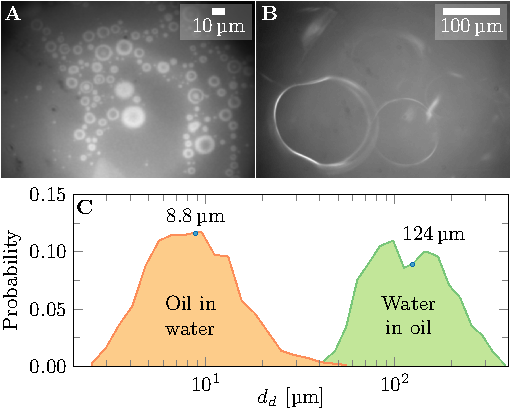
\includegraphics{dropletCombined.pdf}
\caption{A. In-situ microscopic image taken of an o--w suspension of
$\alpha=\SI{60}{\percent}$ in operation at $\omegai/(2\pi)=\SI{8}{\hertz}$. B.
In-situ microscopic image taken of an w--o suspension operating at the same
$\alpha$ and $\omegai$ as A. C. Probability distributions of the typical
diameter of oil drops (in water) and water drops (in oil) for the cases shown
in A and B. Statistics based on $\mathcal{O}(10^3)$ samples, mean values are
indicated above the curves.}
\label{fig:dropletsize}
\end{figure}%
%
A large amount of tiny droplets is identified in each captured frame. The observed rings visible in the droplet images could be due to light diffraction  (as the droplets are only a couple of microns in diameter), or due to the presence of a double emulsion (which has been also observed in Turbulent catastrophic inversion regimes \cite{Piela2008}).
Using a larger acceleration rate (a few minutes start-up time), results in $\nue$ being in
the lower branch, which results in a lower torque value compared to the single phase case. From the typical image shown in \reff{fig:dropletsize}B it is
already evident that for w--o, the droplets are considerably larger. The deformability is also obviously affected: o--w droplets are mostly spherical while the w--o droplets are commonly seen with larger degree of deformation. 
To characterize the droplet size distribution we collected $\mathcal{O}(10^3)$ samples for each type (o--w and w--o) and 
calculated the probability distribution shown in \reff{fig:dropletsize}C.
Water droplets are roughly $14\times$ larger in diameter as compared to oil
drops---a staggering $2800\times$ larger in volume.
Using $d_d$ we calculate the Weber number, $\text{We}=\rho u'^2 d_d / \gamma$,
where $\rho$ is the density of the mixture and $u'$ velocity fluctuations.
The Weber number of the o--w MSE is $\text{We}_{o\text{--}w}=0.01$, while for the
w--o case this is more than an order of magnitude larger,
$\text{We}_{w\text{--}o}=0.16$ but still below unity, a requirement found for bubble
drag reduction\,\cite{vandenBerg2007, Verschoof2016}.
% in context with flow scales
The size of the droplets are linked to the underlying flow structures and a
first guess is generally the Kolmogorov length scale:
$\eta_K=\left(\nue^3/\epsilon \right)^{1/4}$, where $\epsilon$ is the
turbulent energy dissipation. 
From this relation we find \SI{46}{\micro\metre} and \SI{13}{\micro\metre} for
the o--w and w--o case respectively.
These values are both quite off, but this relation does not take into account
interfacial tensions and assumes homogeneous isotropic turbulence.
The scaling from Hinze\,\cite{Hinze1955} does take into account the
interfacial tensions:
\begin{align}
d_{d,\text{max}} \approx 0.725 \left(\rho/\gamma\right)^{-3/5} \epsilon^{-2/5}.
\end{align}
Unfortunately, using the Hinze relation straight away, results in overestimated
droplets, with dimensions above a millimeter.
We can however, use this relation to calculate $\epsilon$ required to find a
similar size of droplets, which showed that $\epsilon$ should be at least
$\mathcal{O}(10^2)$ times larger.
The dissipation of turbulent energy is much larger close to the boundaries as
compared to the bulk.
In simulations at a slightly lower $\Ta$, $\epsilon$ was found to be
approximately $350\times$ larger than in the bulk\,\cite{Zhu2017}.
It is therefore plausible that close to boundaries, $\epsilon$ is large
enough and this would infer that these droplets are mostly generated at
these boundaries.
% asymmetry
However, since such an argument is based solely on surface energies, it should be symmetric, i.e. applicable both for o--w and for w--o droplets identically. We therefore cannot explain such a large asymmetry in droplet
sizes between branches. We speculate that the origin of the asymmetry could be found in the existence of electrical double layers when the continuous medium is polar and conductive (o--w)\,\cite{Gu1998, Eastoe2007}. The presence of certain interfacial electrical charges at the o--w emulsion would hinder coalescence and facilitate break-up. Consequently, the addition of salt to the water phase can be a method to alter drastically the dynamics of the system, opening ways to test this hypothesis in the future. \\
% summary
\ifdefined\thesissections%
\section{Summary}%
\fi%
\indent To summarize, in this work we have studied the flow of meta-stable emulsions with oil volume fractions between $\alpha=0$--$\SI{100}{\percent}$ on a wall boundary in an intensely sheared rotating flow. Exploiting the known scaling of the ultimate regime of Taylor--Couette flow, an effective viscosity of the emulsion can be calculated, and thereby using the TC apparatus as a rheometer far beyond the conventional regime.  
With water as the continuous phase, the addition of oil droplets increases the drag of the system. Interestingly, drag is reduced when the water is injected in a continuous oil phase. 
At a critical volume fraction, a \emph{catastrophic} phase inversion takes place, which dramatically changes the rheological properties.   
Using an in-situ optical microscopy setup, we were able to obtain droplet size distributions while flowing in the TC system. This showed that the w--o droplets are $14\times$ larger than o--w droplets, deformable, and therefore showing a similar drag reduction mechanism as for bubbly drag reduction\,\cite{vandenBerg2007, Verschoof2016}.  
The asymmetry found in the droplet size distribution explains the different rheological response of the system, and it is a truly surprising example of how microscopic phenomena can influence critically the macroscopic behavior of the global system. Our results demonstrate that by tweaking the volume fractions of two immiscible fluids can result in major energetic reductions.  However, exceeding a critical volume fraction can turn this benefit to an energetic disaster.
%
\graphicspath{{fig/}}

